\chapter{B-Spline Computation and Generation}
\label{ch:BSplines}

B-Splines are becoming increasingly important in the field of robotics. This work has discussed the application of B-Splines for a trajectory tracking controller for an eVTOL aircraft. 
B-Splines are piecewise polynomial functions with smooth transition between each piecewise segment.
The degree of smoothness depends on the degree of B-Spline involved.
B-Splines have several advantages over other function representations. 
B-Splines maintain locality, where each control point only controls a finite section of the output, instead of the entire output. 

As the number of applications for B-Splines increases, the computational burden for the generation of B-Splines also increases. 
While they have a relatively low computational burden for a single application, many of the new applications of B-Spline generation may include real time computation, updating, and optimization.

Uniform B-Splines are B-Splines where all basis functions are only time shifted versions of each other.
This is in opposition to clamped B-Splines which use modified basis functions at end points so the B-Spline will be guaranteed to start or stop at a particular point.
To prevent needless repetition of what already exists in the 2025 paper, the majority of the derivations must be referenced only. 

\section{B-Spline Background}

B-Splines can be constructed using the following formula:

\begin{align}
    \bs{p}(t) = \sum_{m=0}^{M+d-1} \bs{c}_m \hat{b}_m^d(t, \bs{k}),
\end{align}

Where $\hat{b}_m^d(t, \bs{k})$ are the time shifted basis functions of degree $d$, given the knot sequence $\bs{k}$. The knot sequence $\bs{k}$ scales the time spacing of the basis function, which means that adjusting the knot sequence adjusts the standard basis function, which can be helpful for edge cases in robotics. The control points $\bs{c}_m$, scale the basis functions to stitch together the final spline. The dimension of the control point $\bs{c}_m$ determines the dimension of the B-Spline, where a 1D $\bs{c}_m$ will create a 1D B-Spline, and so forth.

This paper uses only uniform B-Splines. 
In a uniform B-Spline, the knot points are all uniformly spaced apart. 
If the knot points are all uniformly spaced apart with a spacing of $1$, the basis functions will be defined recursively using the following equations:

\begin{align}
b^0(t) &= \begin{cases} 1 & \text{~if~} 0 \leq t \leq 1 \\ 
 						0 & \text{~otherwise} 
 					   \end{cases},
	\label{eq:uniform_central_basis_0}\\	
b^d(t) &= \left(\frac{t}{d}\right) b^{d-1}(t) + \left(\frac{(d+1)-t}{d}\right) b^{d-1}(t-1).
	\label{eq:uniform_central_basis_d}  
\end{align}

The basis functions with uniform spacing of $1$ are shown in Fig. \ref{fig:central_basis_functions}. If the knot point spacing is $\alpha$, simply replace $t$ with $\frac{t}{\alpha}$, which will scale the basis functions accordingly in the time domain. Uniform B-Splines are particularly useful, because their basis function remains the same for all copies. If all basis functions are the same for a particular B-Spline implementation, it is possible to store that function numerically in a lookup table, for ultra fast implementation. Since they are all the same we will rewrite the symbol for basis functions as: $b^d(t) = \hat{b}_m^d(t, \bs{k})$. 

\begin{figure}[htb]
  \centering
  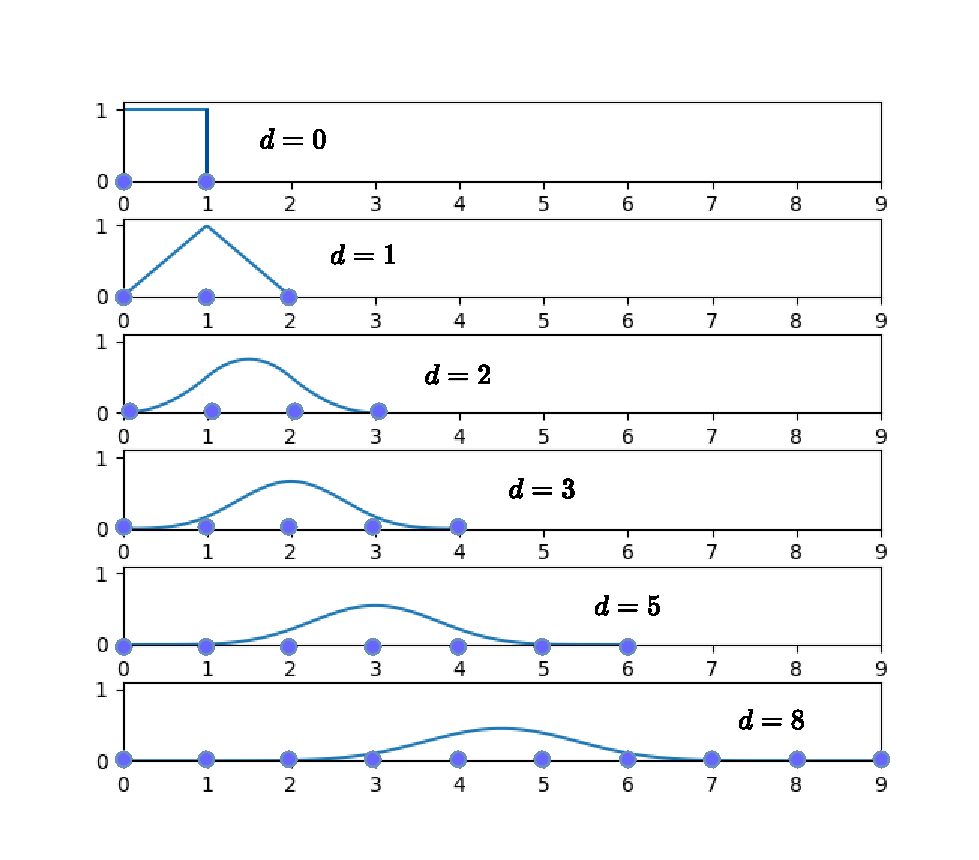
\includegraphics[width=0.8\linewidth]{figs/chap3/central_basis_unclamped.pdf}
  \caption{Central basis functions for different degrees $d$.}
  \label{fig:central_basis_functions}  
\end{figure}

The 

\subsection{Finite Support}

Each basis function is nonzero only on a finite time interval. For example the basis function for the uniform, $1$ spaced, degree 1 Bspline is:

\begin{align}
    b^1(t) &= \begin{cases} t & \text{~if~} 0 \leq t \leq 1 \\ 
 						2-t & 1 \leq t \leq 2 \\
 						0 & \text{~otherwise}
 					    \end{cases}
\end{align}

This basis function is zero outside of the interval $[0,2]$, and similar rules apply to basis functions of any other degree. Recall that the definition for a uniform B-Spline has become:

\begin{align}
    \bs{p}(t) = \sum_{m=0}^{M+d-1} \bs{c}_m b^d(t-m+d), \quad t\in[0,M]
\end{align}

Each term in this sum is a control point $\bs{c}_m$ times a time shifted basis function $b^d(t-m+d)$, where $m$ iterates from $0$ to $M+d-1$. Each control point modifies a time shifted and overlapped copy of the exact same basis function. A figure of overlapped copies of the same basis functions are shown in Fig. \ref{fig:uniform_basis_functions}.

\begin{figure}[htb]
  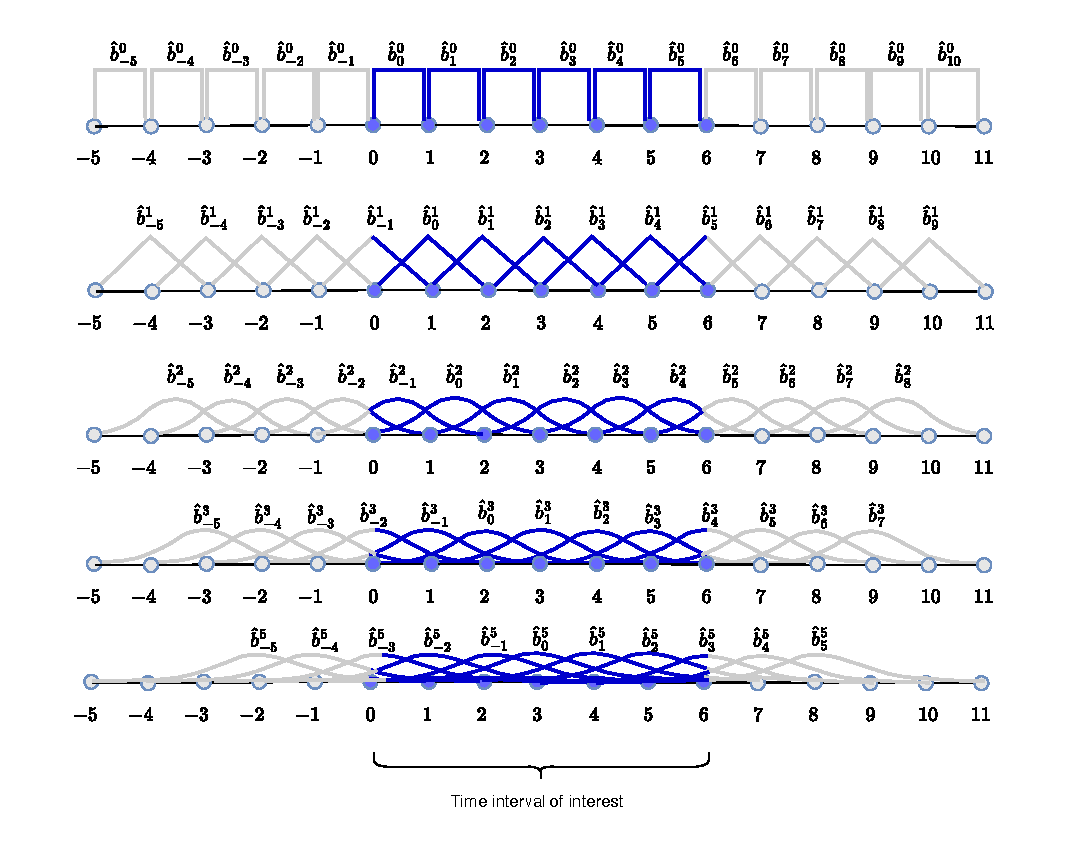
\includegraphics[width=\linewidth]{figs/chap3/uniform_basis_functions.pdf}
  \caption{Uniform basis functions of degree $d=0, 1, 2, 3, 5$ for knot vector $\bs{k}_{M=6}^{\bar{d}=5}$}
  \label{fig:uniform_basis_functions}  
\end{figure}

This means that each control point is assigned to one basis function copy, and scales it accordingly. The size of each time-shifted basis function is finite and only covers a small section of the whole B-Spline. Therefore, modification of one control point only affects local area around that B-Spline, and not its entirety. This is one of the great advantages of B-Splines, that modifications may be made in one area without affecting another if it is sufficiently far away. This principle is illustrated in Fig. \ref{fig:BasisFunctionsConnection}. 


This example uses $d=1$ and $M=9$, which is to say there are $9$ intervals of interest the B-Spline is defined over. The knot vector is given, with uniform spacing of $1$ as: 

\begin{align}
        \bs{k}^{d=1}_{M=9} =
    \begin{bmatrix}
        -1 & 0 & 1 & 2 & \hdots & 7 & 8 & 9\\
    \end{bmatrix}
\end{align}

Two sets of $d+M = 1+9=10$ control points are given for the same knot vector. These are:

\begin{align}
    \bs{C}_1 =
    \begin{bmatrix}
        1&2&-1&-0.5&0.5&1.5&3.0 & 5.0 & 4.5 & -3.0
    \end{bmatrix}\\
    \bs{C}_2 =
    \begin{bmatrix}
        1&2&-1&-0.5&0.5&-2.0&3.0 & 5.0 & 4.5 & -3.0\\
    \end{bmatrix}
\end{align}

The only difference is that for $\bs{C}_1$, the value at index $5$ is $1.5$, while for $\bs{C}_2$, the value at index $5$ is $-2.0$. Notice that this altered control point only modifies the B-Spline function on the interval $[4.0,6.0]$; the rest of the spline remains the same.

\begin{figure}
    \centering
    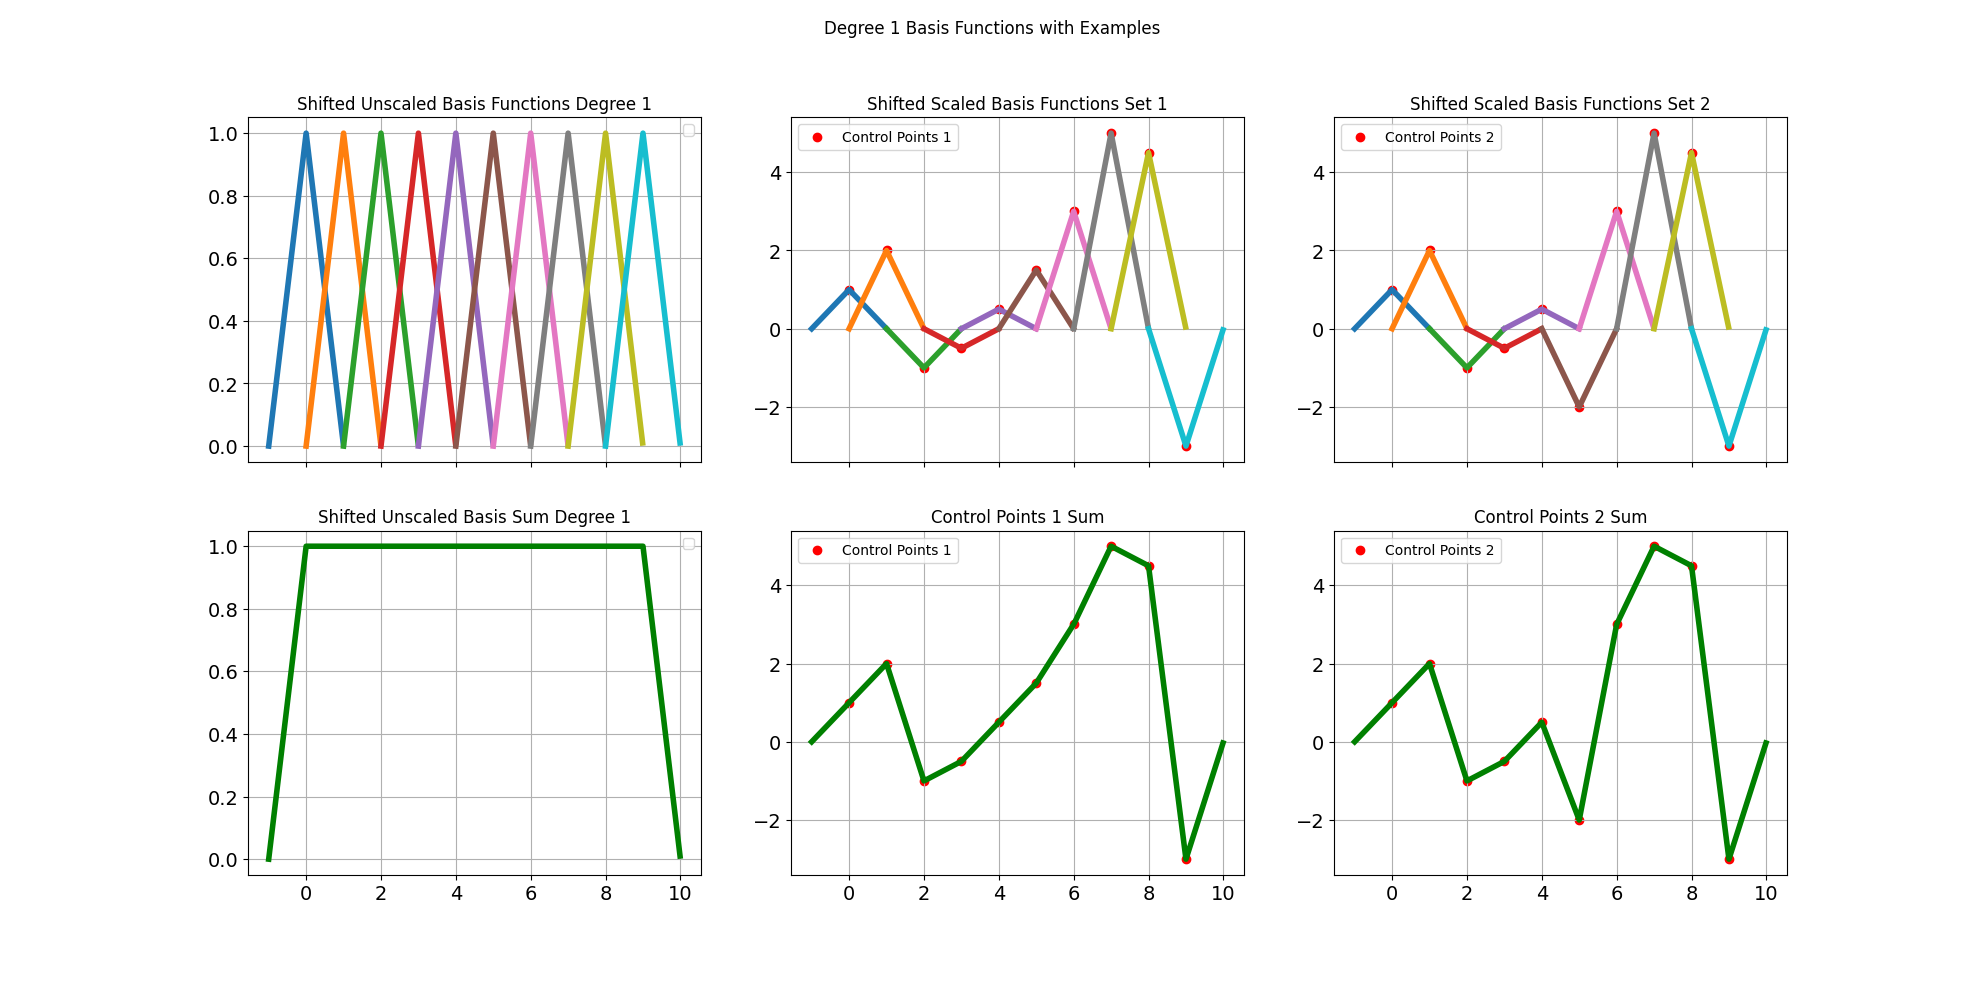
\includegraphics[width=1.0\linewidth]{figs/chap3/mainPlot.png}
    \caption{Degree 1 B-Spline Formation. Top left is a series of time shifted degree 1 B-Spline basis functions overlapping. Bottom left is the sum of all basis functions from the above. Top middle plots the control points in red, with the correspondingly scaled and time shifted basis functions. Bottom middle is the sum of all basis functions. Right plots are identical to middle plots, except with the index $5$ control point changed from $1.5$ to $2$.}
    \label{fig:BasisFunctionsConnection}
\end{figure}

For the specific implementation used to generate this plot, the B-Spline basis function was sampled beforehand into a lookup table, and stitched together using the control points.

\section{Matrix Representation of B-Splines}
\label{sec:BSplineMatrixRepresentation}

Recall that the summation formula for a B-Spline is given as:

\begin{align}
    \bs{p}(t) &= \sum_{m=0}^{M+d-1} \bs{c}_m b^d(t-m+d)
\end{align}

This definition may be converted from a sum to a matrix form as

\begin{align}
    \bs{p}(t) =
    \begin{bmatrix} \bs{c}_0 & \dots & \bs{c}_{M+d-1}\end{bmatrix}
		\begin{bmatrix}
			b^d(t+d) \\
			b^d(t+d-1) \\
                \vdots \\
			b^d(t-M+1)
		\end{bmatrix} \\
	= \bs{C} \bs{b}^d_M(t)
\end{align}

Where

\begin{align}
	\bs{C} &\doteq \begin{bmatrix} \bs{c}_0 & \dots & \bs{c}_{M+d-1} \end{bmatrix}
	\\
	\bs{b}^d_M(t) &\doteq \begin{bmatrix}
			b^d(t+d) \\
			b^d(t+d-1) \\
			\vdots \\
			b^d(t+1) \\
			b^d(t) \\
			b^d(t-1)\\
			\vdots \\
			b^d(t-M+1)
		\end{bmatrix},
\end{align}

This form simply stacks each shifted basis function into a vector. For any given time $t$, those shifted functions are simply evaluated to produce a number for each entry. That vector is multiplied by the control point and that produces the evaluated position $\bs{p}(t)$. 

\section{Derivatives of Uniform B-Splines}

It is shown in Lemma 1.13 in \citeauthor{beard2025BSplines} \cite{beard2025BSplines} that the derivative of a B-Spline is given as:

\begin{align}
    \frac{db^d}{dt}(t) = b^{d-1}(t) - b^{d-1}(t-1).
\end{align}

Representing this in matrix form simply requires subtraction between components the two basis function vectors of degree $d-1$. This is accomplished using the derivative matrix $D_M^d$ as follows:

\begin{align}
    \frac{d\bs{p}}{dt}(t) = \bs{C} D_M^{d} \bs{b}_M^{d-1}(t),\\
    D_M^{d} = 
    \begin{bmatrix}
        \bs{0}_{1\times(M+d-1)} \\ \bs{I}_{M+d-1} 
    \end{bmatrix} 
 	-\begin{bmatrix}
        \bs{I}_{M+d-1} \\ \bs{0}_{1\times(M+d-1)} 
    \end{bmatrix},
\end{align}

As an example, if $M=4$ and $d=1$, the derivative basis vector is:

\begin{align}
    \bs{b}^0_4(t) =
    \begin{bmatrix}
        b^0(t)\\
        b^0(t-1)\\
        b^0(t-2)\\
        b^0(t-3)\\
    \end{bmatrix}
\end{align}

and the derivative matrix is:

\begin{align}
    D_M^d =
    \begin{bmatrix}
        -1 & 0 & 0 & 0\\
        1 & -1 & 0 & 0\\
        0 & 1 & -1 & 0\\
        0 & 0 & 1 & -1\\
        0 & 0 & 0 & 1\\
    \end{bmatrix}
\end{align}

The resulting vector $D_4^1 \bs{b}^0_4(t)$ then becomes:

\begin{align}
    D_4^1 \bs{b}^0_4(t) = 
    \begin{bmatrix}
        -b^0(t)\\
        b^0(t) - b^0(t-1)\\
        b^0(t-1) - b^0(t-2)\\
        b^0(t-2) - b^0(t-3)\\
        b^0(t-3)\\
    \end{bmatrix}
\end{align}

The proof for this property is given after Lemma 1.14 in \citeauthor{beard2025BSplines} \cite{beard2025BSplines}.

\section{Endpoint Constraints}

Note that the same control points $\bs{C}$ relate both position and velocity to their modified basis functions as:

\begin{align}
    \bs{p}(t) = \bs{C} \bs{b}^d_M(t)\\
    \frac{d\bs{p}}{dt}(t) = \bs{C} D_M^{d} \bs{b}_M^{d-1}(t),\\
\end{align}

These can also be put into matrix form for $d=2$ as:

\begin{align}
    \begin{bmatrix}
        \bs{p}(t_i) & \frac{d\bs{p}(t_i)}{dt}
    \end{bmatrix}
	= \bs{C}
    \begin{bmatrix}
        \bs{b}_M^2(t_i) & D^2_M \bs{b}^1_M(t_i) 
    \end{bmatrix}
\end{align}

Where 

\begin{align}
    B_M^2(t) = 
    \begin{bmatrix}
        \bs{b}_M^2(t) & D^2_M \bs{b}^1_M(t) 
    \end{bmatrix}
\end{align}



This demonstrates the relationship between the state of the B-Spline and the evaluation of the basis functions at a particular time. The modified basis functions are already known. If the conditions are known, then it is possible to find the control points using this relationship.

However, this only applies to $d$ control points, given $d$ known conditions. At any given time, most values in the $\bs{b}$ vector will be zero. For each $t$ that is equal to a knot point $k_i$, the nonzero values simply shift down the vector. For example, if $d = 2$ and $M = 4$, $k = [-2, -1, 0, 1, 2, 3, 4, 5, 6]$ $\bs{b}_M^d(t)$ becomes:

\begin{align}
    \bs{b}_4^2(t) =
    \begin{bmatrix}
        b^2(t+2)\\
        b^2(t+1)\\
        b^2(t)\\
        b^2(t-1)\\
        b^2(t-2)\\
        b^2(t-3)\\
    \end{bmatrix}
\end{align}

If we then evaluate this vector for knot points in the interval of interest: $\bs{k} = [0,1,2,3,4]$

\begin{align}
    \bs{b}_4^2(0) =
    \begin{bmatrix}
        0.5\\
        0.5\\
        0.0\\
        0.0\\
        0.0\\
        0.0\\
    \end{bmatrix}
    \quad
    \bs{b}_4^2(1) =
    \begin{bmatrix}
        0.0\\
        0.5\\
        0.5\\
        0.0\\
        0.0\\
        0.0\\
    \end{bmatrix}
    \quad
    \bs{b}_4^2(4) =
    \begin{bmatrix}
        0.0\\
        0.0\\
        0.0\\
        0.0\\
        0.5\\
        0.5\\
    \end{bmatrix}
\end{align}

Notice that the nonzero values simply shift down the vector. We call these nonzero

The same effect occurs with the derivative vectors from $D_M^d b_M^{d-1}(t)$. For the same example, if $t=0$:

\begin{align}
    \bs{b}^1_4(t) =
    \begin{bmatrix}
        b^1(t+1)\\
        b^1(t)\\
        b^1(t-1)\\
        b^1(t-2)\\
        b^1(t-3)\\        
    \end{bmatrix}
\end{align}

If $t=0$

\begin{align}
    \bs{b}^1_4(0) =
    \begin{bmatrix}
        1\\
        0\\
        0\\
        0\\
        0\\
    \end{bmatrix}
\end{align}


\begin{align}
    D^2_4 \bs{b}^1_4(0) = 
    \begin{bmatrix}
        -1\\
        1\\
        0\\
        0\\
        0\\
        0\\
    \end{bmatrix}
\end{align}

The matrix $B_4^2(0)$ then becomes:

\begin{align}
    \begin{bmatrix}
        0.5 & -1\\
        0.5 & 1\\
        0.0 & 0\\
        0.0 & 0\\
        0.0 & 0\\
        0.0 & 0\\
    \end{bmatrix}
\end{align}

It turns out that the top, nonzero section will simply shift down for each subsequent shift in $t$. We denote the nonzero section to be $\hat{B}_4^2$, which is time invariant. This simplifies the control point relationship to be:

\begin{align}
    \begin{bmatrix}
        \bs{p}(0) & \frac{d\bs{p}(0)}{dt}
    \end{bmatrix}
	= \bs{C}_{0:1}
    \hat{B}_4^2
	= \bs{C}_{0:1}
    \begin{bmatrix}
        0.5 & -1.0\\
        0.5 & 1.0\\
    \end{bmatrix}
\end{align}

Given the position and velocity conditions, it is trivial to find the initial control points using a matrix inverse as:

\begin{align}
    \bs{C}_{0:1} =
    \begin{bmatrix}
        \bs{p}(0) & \frac{d\bs{p}(0)}{dt}
    \end{bmatrix}
    (\hat{B}_4^2)^{-1}
	=
    \begin{bmatrix}
        \bs{p}(0) & \frac{d\bs{p}(0)}{dt}
    \end{bmatrix}
    \begin{bmatrix}
        0.5 & -1.0\\
        0.5 & 1.0\\
    \end{bmatrix}^{-1}
\end{align}


This process can be implemented for both initial and final conditions as

 \begin{align*}
 	\bs{S} &\doteq \begin{bmatrix}\bs{p}(0) & \frac{d\bs{p}(0)}{dt} & \dots & \frac{d^\ell\bs{p}(0)}{d^\ell t} \end{bmatrix} 	\\
 	\bs{E} &\doteq \begin{bmatrix}\bs{p}(M) & \frac{d\bs{p}(M)}{dt} & \dots & \frac{d^\ell\bs{p}(M)}{d^\ell t} \end{bmatrix}.
 \end{align*}

 Segment the spline control points into the first and last $d$-elements as
 \[
 \bs{C} = \begin{bmatrix}\bs{C}_{1:d} & \bs{C}_{(d+1):(M)} & \bs{C}_{(M+1):(M+d)} \end{bmatrix},
 \]
 and define the matrix
 \[
 B_M^d(t) \doteq \begin{bmatrix} 
 \bs{b}^d_M(t) & D_M^d \bs{b}^{d-1}_M(t) & \dots & D_M^d D_M^{d-1}\dots D_M^{d-\ell+1} \bs{b}^{d-\ell}_M(t)
 				\end{bmatrix},
 \]

 Then we may find the start and end control points given the start and end conditions $\bs{S}$ and $\bs{E}$. This work work at any point, as long as the conditions at that point are known. 

\begin{align}
    \bs{C}_{1:d} = \bs{S} \left(\hat{B}_M^d(0)\right)^{-1}\\
    \bs{C}_{M+1:M+d} = \bs{E} \left(\hat{B}_M^d(M)\right)^{-1}
\end{align}


\section{Minimum Snap Trajectory}

The above formula enables us to generate initial and final control points for the B-Spline, but it says nothing about the control points in between. While there are countless options for placement of the control points between start and finish, one particularly useful method is a minimum snap trajectory. Snap is the third derivative of position, after velocity and acceleration. A minimum snap trajectory finds the trajectory with the lowest integral of snap, given the initial conditions $\bs{S}$ and $\bs{E}$. This is given as:

 \begin{equation}
 	\label{eq:min_integral_of_norm}
 	\begin{aligned}
 	&\min_{\bs{C}} trace {\bs{C} W_M^{d}(\bs{\rho}) \bs{C}^\top} \\
 	&\text{subject to } \: \bs{C} \begin{bmatrix} B_M^d(0) & B_M^d(M) \end{bmatrix} = \begin{bmatrix} \bs{S} & \bs{E} \end{bmatrix}. 
 	\end{aligned}
 \end{equation}

 Where $W_M^{d}(\bs{\rho})$ is a mixing matrix that will be defined later.

\section{Integral objective}

The following section summarizes the derivation for minimum snap control points. While this section highlights the most important equations, the full derivation is found in \citeauthor{beard2025BSplines} \cite{beard2025BSplines}.

The objective for creating control points that minimize the integral of an $\ell^{th}$ derivative, which in our case is $3^{rd}$ derivative, is given in section $2.6$ of \cite{beard2025BSplines} as:

\begin{equation}
    \label{eq:integral_constraint}
    \bs{C}^\ast = \arg\min_{\bs{C}} \int_0^M \sum_{\ell=0}^L \left( \rho^\ell \norm{\bs{p}^{\ell}(t)}^2\right) \, dt
\end{equation}

Finding the generalized $\ell^{th}$ order derivative of a B-Spline is possible using the following equations:

Define
 \[
 D_M^{d,\ell} \defeq D_M^d D_M^{d-1}\cdots D_M^{d-\ell}
 \]
 implying that 
 \begin{align*}
 	\bs{p}^{\ell}(t) &= \bs{C} D_M^{d,\ell-1} 	\bs{b}_M^{d-\ell}(t).
 \end{align*}

We define $\bs{\rho}$ as a vector of size $L$ coefficients that are selected by the user to weight which derivative terms are the most significant for the trajectory.

If we define the matrices $S_M^k$ and $W_M^{d,l}$ as:

\begin{align*}
    S_M^k &\defeq \int_0^M 	\bs{b}_M^{k}(t) {\bs{b}_M^{k}(t)}^\top \, dt \\
    W_M^{d,\ell} &\defeq D_M^{d,\ell-1} S_M^{d-\ell} {D_M^{d,\ell-1}}^\top,
\end{align*}

Then we may define:

\begin{align}
    W_M^{d}(\bs{\rho}) \defeq \sum_{\ell=0}^L \rho^\ell W_M^{d,\ell}.
\end{align}

This matrix essentially creates an objective function by relating the control points $\bs{C}$ to the specified derivative we want to minimize over the entire path. From this, a solution may be derived.

A lengthy derivation follows in section 2.6 in \cite{beard2025BSplines}, which will not be repeated here. It turns out that there is an analytical solution to this problem. First, if we take the singular value decomposition of two $B$ matrices as:

\begin{align}
    B^d_{M,SE} = 
    \begin{bmatrix} 
        B_M^d(0) & B_M^d(M) 
    \end{bmatrix} =
    \begin{bmatrix}
        U_1 & U_2
    \end{bmatrix}
    \begin{bmatrix}
        \Sigma \\ 
        \bs{0} 
    \end{bmatrix} 
    V^\top,
\end{align}


Then the analytical solution to the control points $\bs{C}^*$ for a minimum snap trajectory are given as:

\begin{align}
    \bs{C}^\ast = 
    \begin{bmatrix} 
        \bs{S} & \bs{E} 
    \end{bmatrix}
    Q_M^{d}(\bs{\rho})
\end{align}

Where
\begin{align}
     Q_M^{d}(\bs{\rho}) = V \Sigma^{-1} U_1^\top \left( I - W_M^{d}(\bs{\rho}) U_2 (U_2^\top W_M^{d}(\bs{\rho}) U_2 )^{-1} U_2^\top \right)
\end{align}

\section{Contributions}

The unique contribution presented in this section is an efficient method of generating and storing look up tables to generate $Q_M^{d}(\bs{\rho})$ as efficiently as possible. Notice that $Q_M^{d}(\bs{\rho})$ is a function of $M$ and $d$, and with a sufficiently large enumeration of values for $M$ and $d$, it becomes possible to have a matrix lookup for each value. While the user defined scaling vector $\rho$ makes it impossible to store $Q_M^d(\bs{\rho})$ directly, it is possible to store the components matrices of $Q_M^d(\bs{\rho})$ as look-up tables to dramatically reduce computation time. 

In this lookup table, we generated tables for degrees $0$ to $5$ inclusive, and number of intervals of interest $M$ up to $M=100$.

\subsubsection{B Matrices}

Recall that the definition for the matrix used in the singular value decomposition is:

\begin{align}
    B^d_{M,SE} =
    \begin{bmatrix} 
        B_M^d(0) & B_M^d(M) 
    \end{bmatrix}
\end{align}

Where $B_M^d(t)$ is:

\begin{align}
B_M^d(t) \doteq 
    \begin{bmatrix} 
        \bs{b}^d_M(t) & D_M^d \bs{b}^{d-1}_M(t) & \dots & D_M^d D_M^{d-1}\dots D_M^{d-\ell+1} \bs{b}^{d-\ell}_M(t)
 	\end{bmatrix},
\end{align}

For degrees $0$ to $5$ and all valid $M$ up to $M=100$, a $B^d_{M,SE}$ is generated and its singular value decomposition is found. Each component is unique to a particular $M$ and $d$ as:

\begin{align}
    B^d_{M,SE} =
    \begin{bmatrix}
        U^d_{M,1} & U^d_{M,2}
    \end{bmatrix}
    \begin{bmatrix}
        \Sigma^d_M \\ 
        \bs{0} 
    \end{bmatrix} 
    V^{d,\top}_M
\end{align}

These components are saved into their own corresponding lookup tables, with a key of $d$ and $M$ for each component. Notice that the first three components of $Q_M^d(\rho)$ are $V \Sigma^{-1} U_1^\top$, which is the left pseudoinverse of $B^d_{M,SE}$, which is also stored in a lookup table for even faster computation. This is represented as $(B^d_{M,SE})^+ = V \Sigma^{-1} U_1^\top$ When finding a particular $Q_M^d(\rho)$, $(B^d_{M,SE})^+$ and $U_2$ are read from memory.

\subsubsection{Y Z Lookup Tables}

The problematic portion of this formula is the part related to the inverse:

\begin{align}
    W_M^{d}(\bs{\rho}) U_2 (U_2^\top W_M^{d}(\bs{\rho}) U_2 )^{-1} U_2^\top
\end{align}

This involves a lot of matrix multiplication, and a matrix inverse, which we desire to minimize as much as possible. The precompute as much of this as possible, we defined some terms as:

\begin{align}
    Y^d_M(\bs{\rho}) = W_M^{d}(\bs{\rho}) U^d_{2,M}
\end{align}

\begin{align}
    Z^d_M(\bs{\rho}) = (U^{d}_{2,M})^\top W_M^{d}(\bs{\rho}) U^d_{2,M}
\end{align}

Recall the definition for $W_M^{d}(\bs{\rho})$:

\begin{align}
    W_M^{d}(\bs{\rho}) \defeq \sum_{\ell=0}^L \rho^\ell W_M^{d,\ell}.
\end{align}

Which may be substituted

\begin{align}
    Y^d_M(\bs{\rho}) = \sum_{\ell=0}^L \rho^\ell W_M^{d,\ell} U^d_{2,M}\\
    Z^d_M(\bs{\rho}) = (U^{d}_{2,M})^\top \sum_{\ell=0}^L \rho^\ell W_M^{d,\ell} U^d_{2,M} = \sum_{\ell=0}^L \rho^\ell (U^{d}_{2,M})^\top  W_M^{d,\ell} U^d_{2,M}
\end{align}

If we make the following definitions:

\begin{align}
    Y^{d,l}_M = W_M^{d,\ell} U^d_{2,M}\\
    Z^{d,l}_M = (U^{d}_{2,M})^\top  W_M^{d,\ell} U^d_{2,M}
\end{align}

The original equations simplify to:

\begin{align}
    Y^d_M(\bs{\rho}) = \sum_{\ell=0}^L \rho^\ell Y^{d,l}_M\\
    Z^d_M(\bs{\rho}) = \sum_{\ell=0}^L \rho^\ell Z^{d,l}_M
\end{align}

Lookup tables are created over all applicable values for $d$, $l$, and $M$ for $Y^{d,l}_M$ and $Z^{d,l}_M$. In the generator program, finding $Q_M^{d}(\bs{\rho})$ turns into the following equation:

\begin{align}
    Q_M^{d}(\bs{\rho}) = (B^d_{M,SE})^+ \left(I - \sum_{\ell=0}^L \rho^\ell Y^{d,l}_M \left(\sum_{\ell=0}^L \rho^\ell Z^{d,l}_M\right)^{-1} U_2^\top \right)
\end{align}

And the equation for finding the remaining control points remains:

\begin{align}
    \bs{C}^\ast = 
    \begin{bmatrix} 
        \bs{S} & \bs{E} 
    \end{bmatrix}
    Q_M^{d}(\bs{\rho})
\end{align}

If a user's mixing vector $\bs{\rho}$ is known beforehand and does not change, the entire $Q_M^{d}(\bs{\rho})$ matrix can be computed once, which would further reduce computation time. 

\section{Results}

We begin with a spline generated using parameters

\begin{align}
    d = 3\\
    M = 15\\
    \rho = \left[1.0, 1.0, 1.0\right]
\end{align}

and a set of 2D conditions as

\begin{align}
    p(0) =
    \begin{bmatrix}
        0.0\\
        0.0
    \end{bmatrix}
    \quad
    \frac{d}{dt}p(0) =
    \begin{bmatrix}
        25.0\\
        0.0
    \end{bmatrix}
    \quad
    \frac{d^2}{dt^2}p(0) =
    \begin{bmatrix}
        0.0\\
        -10.0
    \end{bmatrix}\\
    p(15) =
    \begin{bmatrix}
        200.0\\
        -100.0
    \end{bmatrix}
    \quad
    \frac{d}{dt}p(15) =
    \begin{bmatrix}
        -2.0\\
        -15.0
    \end{bmatrix}
    \quad
    \frac{d^2}{dt^2}p(15) =
    \begin{bmatrix}
        4.0\\
        0.0
    \end{bmatrix}
\end{align}.

This was run through a minimum snap trajectory generator, which yielded the plot in Fig. \ref{fig:minimumSnap2D}.
Using the lookup table library, the total generation time for control points was $803.5$ microseconds.

\begin{figure}
    \centering
    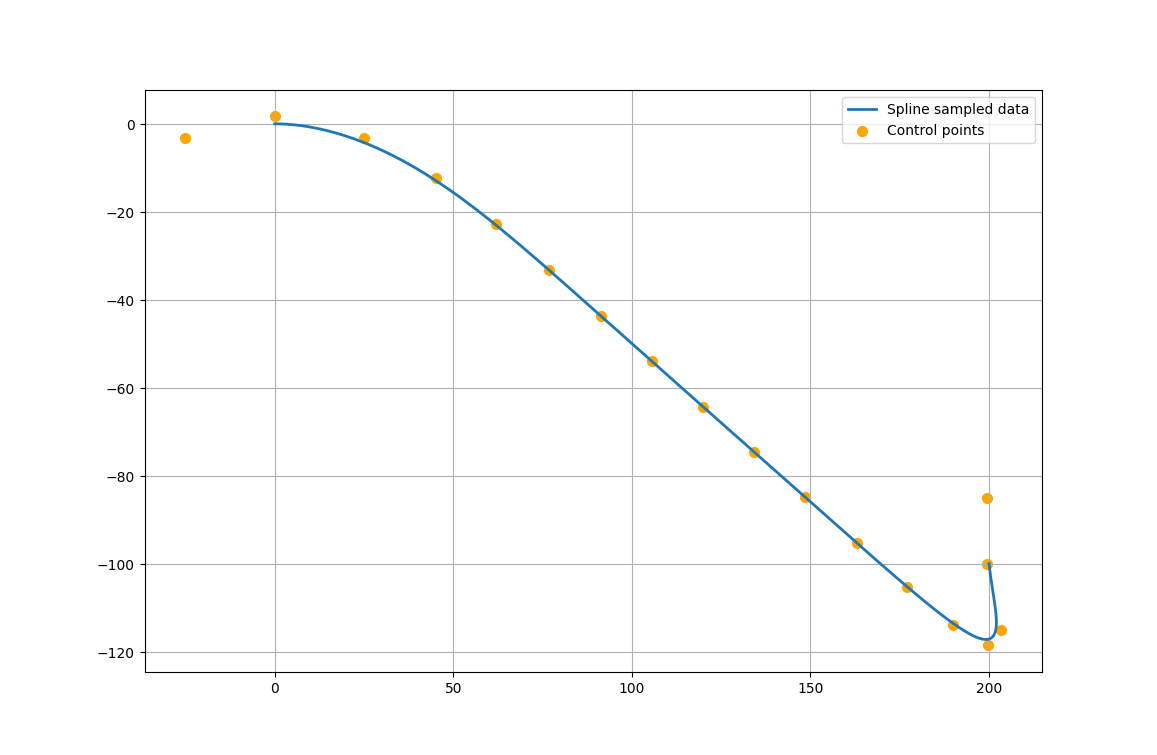
\includegraphics[width=1.0\linewidth]{figs/chap3/2DPlot.png}
    \caption{2D plot of minimum snap trajectory with control points, using initial and final conditions.}
    \label{fig:minimumSnap2D}
\end{figure}

The same set of parameters for $\rho$, $d$, and $M$ with the conditions of 


\begin{align}
    p(0) =
    \begin{bmatrix}
        0.0\\
        0.0\\
        -100.0
    \end{bmatrix}
    \quad
    \frac{d}{dt}p(0) =
    \begin{bmatrix}
        25.0\\
        0.0\\
        0.0
    \end{bmatrix}
    \quad
    \frac{d^2}{dt^2}p(0) =
    \begin{bmatrix}
        0.0\\
        0.0\\
        0.0
    \end{bmatrix}\\
    p(15) =
    \begin{bmatrix}
        199.68\\
        223.4\\
        -100.0
    \end{bmatrix}
    \quad
    \frac{d}{dt}p(15) =
    \begin{bmatrix}
        16.64\\
        18.65\\
        0.0
    \end{bmatrix}
    \quad
    \frac{d^2}{dt^2}p(15) =
    \begin{bmatrix}
        0.0\\
        0.0\\
        0.0
    \end{bmatrix}
\end{align}.

These conditions yielded the 3D B-Spline in Fig. \ref{fig:minimumSnap3D}. 
Using the lookup table library, the total control point generation time was $1.134$ milliseconds.

\begin{figure}
    \centering
    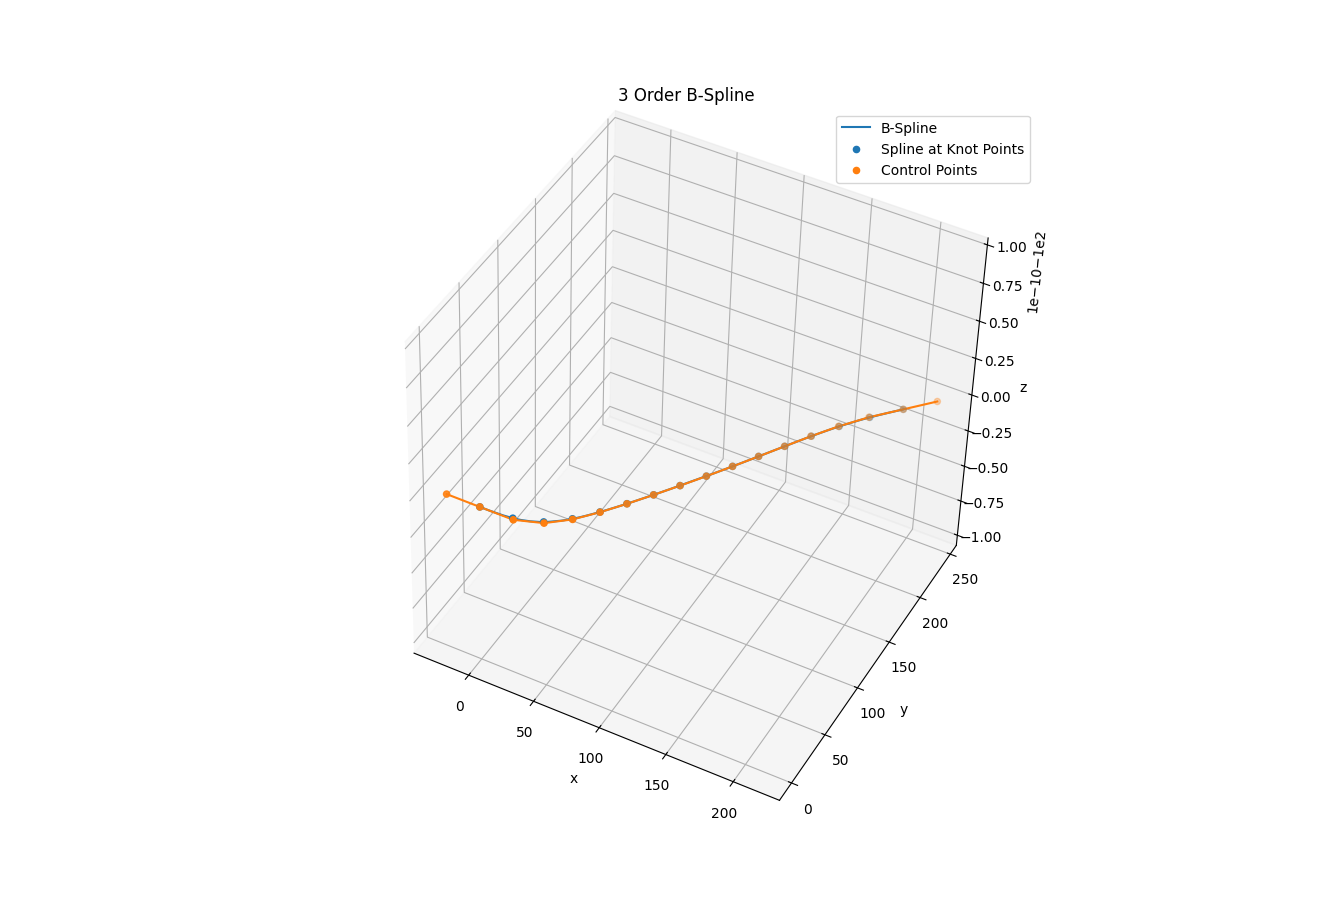
\includegraphics[width=1.0\linewidth]{figs/chap3/3DPlot.png}
    \caption{3D plot of minimum snap trajectory with control points, using initial and final conditions.}
    \label{fig:minimumSnap3D}
\end{figure}

\subsection{Conclusion}

The lookup table method described in this section is implemented in an public repository as \href{https://github.com/byu-magicc/eVTOL_BSplines}{eVTOL\_BSplines}. 
It was implemented in Python, without any C++ or Rust wrappers; creating such wrappers in the future may further increase computational speed. 

One future improvement may include additional lookup tables for $Q_M^d(\bs{\rho})$ for common values of $\bs{\rho}$. 
Recall that $\rho$ sets the relative importance of position, velocity, and acceleration for the B-Spline ouput.
Although there are an infinite number of possible $\rho$ vectors, several common ones may be stored as their own lookup tables, including

\begin{align}
    \rho_0 = \left[1,1,1\right],
    \rho_1 = \left[1,0,0\right]\\
    \rho_2 = \left[0,1,0\right]\\
    \rho_3 = \left[0,0,1\right]\\
\end{align}

among many other possibilities.

It is worth noting that minimum snap trajectories were not used in the other sections of this paper. 
They were originally intended for the takeoff and landing trajectories for the eVTOL section, but additional constraints limited their use. 
Using only start and end position, velocity, and acceleration conditions, it is not possible to create an entirely smooth trajectory for the VTOL.
However, it may be possible to use minimum snap trajectories to stitch together larger trajectories from smaller groups of conditions.
A future area of research would be optimizing sets of intermediate conditions, interpolated with minimum snap trajectories, to develop more complex UAV trajectories.
